%!TEX root = ../main.tex
\chapter{Introduction\label{chap:introduction}}
The field of mobile robotics has undergone significant progress in the past decades.
Robots are nowadays capable of performing a wide variety of tasks. 
Such systems can be more efficient than human workers and can replace them in environments that are dangerous for human beings.
One possible application for autonomous robots is the mapping and monitoring of ionizing radiation. 
Radioactive materials are part of our world, and there are several situations when such a need might occur, for example, a disaster in a nuclear power plant or misuse of materials for radiotherapy in medicine. 
To ensure public safety, we need a method for fast and efficient localization of radioactive sources without the presence of human workers.
\acp{UAV} (frequently referred as drones) equipped with appropriate sensors presents a promising solution to this problem.
A group of highly mobile \ac{UAV}s can quickly and autonomously explore large areas and perform measurements needed for precise localization of radioactive sources.

Sensing of ionizing radiation is possible thanks to the variety of sensors, one of which is called the Compton camera.
The Compton camera utilizes the Compton scattering effect, which was discovered by Arthur Compton in 1923 \cite{compton}.
During the Compton scattering, an ionizing photon interacts with an electron and scatters (the photon's direction is changed while part of the photon's energy is transferred to the electron).
This principle allows the Compton camera to not only detect the presence of ionizing particles (as common in intensity-based sensors, such as widely known dosimeters), but also reconstruct a set of possible directions from where the photon arrived to the sensor.
Thanks to innovations in the field of sensory equipment, Compton camera \ac{pix} became small and lightweight enough to be carried by a small \ac{UAV} onboard.

\begin{figure}[!h]
    \centering
  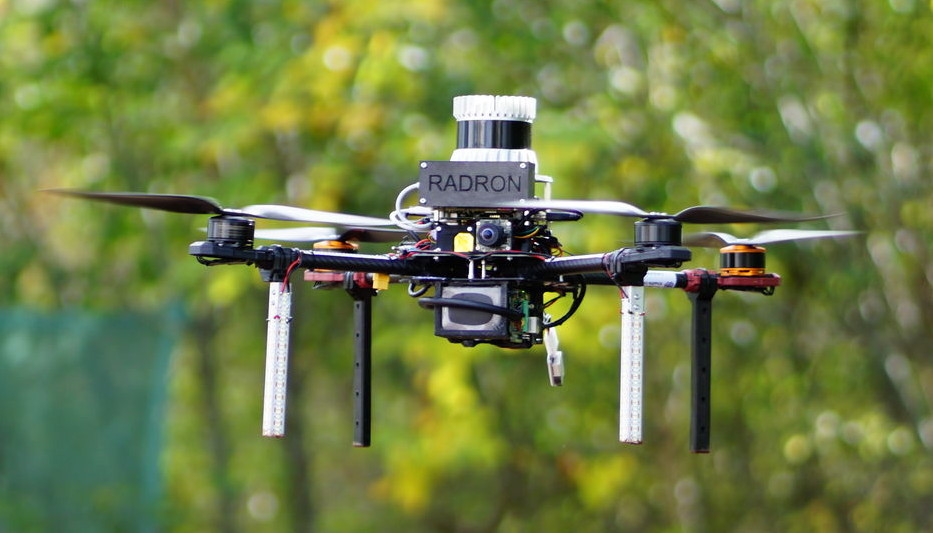
\includegraphics[width=0.7\textwidth]{./fig/photos/uav.jpg}
    \caption{A small T650 multi-rotor UAV equipped with the \ac{pix} sensor. Source: \cite{baca2021gamma}.}
    \label{fig:uavvv}
\end{figure}

This thesis aims to present a method that performs fusion of sensory data from multiple \ac{UAV}s (equipped with the Compton camera sensor) in order to localize multiple sources of ionizing radiation.
The estimation method is based on the \ac{MLEM} algorithm that estimates distribution of sources of ionizing radiation while maximizing likelihood of measured data.
The localization of radioactive sources is performed online during the flight.
Thanks to the online estimation, the group of \ac{UAV}s autonomously adapts its actions accordingly in order to increase the precision of the estimate and minimize the search time.
The presented data fusion method, as well as the high-level search strategy, are tested in simulations and on prerecorded data from real-world experiments.

\section{Related work}
The remote sensing of ionizing radiation is a very broad topic involving many disciplines, such as medicine, astronomy, industry, public safety or robotics.
The overview presented in \cite{radiation_detection_systems_overview} shows various mobile radiation detection systems, sensors and reconstruction methods that were presented in the past decade.
The focus of this thesis is on remote sensing using unmanned vehicles.
Several works describing radiation mapping using robots appeared after 2011 when the biggest radioactive accident in past decades happened in Japan.
The strong earthquake and following tsunami wave caused several leakages of radioactive substances from \ac{FDNPP}.
The contaminated area of the powerplant was explored by \ac{UGV}s (\cite{fuku2012,fuku_compton}) as well as \ac{UAV}s equipped with different radioactivity sensors (\cite{sanada2015, towler2012, Jiang2015, Mochizuki_2017, sato_drone_compton_camera_2018}).

%\subsubsection{Intensity-based methods}
Sensors used for remote monitoring of ionizing radiation can be generally classified into two groups: intensity-based and direction-based.
Intensity-based detectors measure only the number of particles recorded in the sensor (particle flux at the sensor's position), whereas the direction-based detectors can also estimate the direction of ionizing radiation.
The intensity-based detectors are widely used in remote sensing of ionizing radiation..
The distribution of radioactive material is estimated thanks to intensity measurements acquired at different positions.
A group of \ac{UGV}s remotely sensing contaminated indoor area is presented in \cite{fuku2012}.
Radiation mapping of a large-scale area around the \ac{FDNPP} powerplant using an unmanned helicopter equipped with large scintillation intensity-based detectors is shown in \cite{sanada2015} and \cite{towler2012}.
Multi-rotor \ac{UAV}s have been used for remote sensing in \cite{nine_drone_fukushima, ten_remote_sensing_with_uderstanding_uav_ugv} and \cite{eleven_remote_sensing_non_japan}.
In most of the presented experiments, the \ac{UAV}s were following predefined trajectories.
The radiation mapping was done offline after the flight.

A recent paper \cite{mascarich2022} presents a method for radiation mapping in the indoor environment.
The method is based on estimating the gradient of radiation from multiple intensity-based measurements.
The onboard sensors can not only localize the sources of radioactivity but also estimate the energetic spectrum of measured particles and decide which radioactive material is detected.
Moreover, the authors have presented an active search path planning method that plans the movement of the drone in order to improve the quality of measurements and shorten the search time.

Work presented in \cite{stibinger2020} shows a method for radioactivity mapping using intensity-based dosimetric measurements acquired by the same sensor as in this thesis.
Each drone measured intensities in multiple directions while statically hovering at it's current position.
The direction with the highest intensity was chosen as a direction vector towards the source.
These directions vectors acquired at different positions were fused using \ac{LKF}.
However, this method is not designed for the localization of multiple sources of radiation.

This thesis focuses on the direction-based sensor --- the Compton camera.
Radiation mapping around \ac{FDNPP} using an \ac{UAV} equipped with a Compton camera is presented in \cite{Jiang2015, Mochizuki_2017, sato_drone_compton_camera_2018}.
In all cases, the platforms were hovering for a certain time above the predefined positions and the radiation images were reconstructed offline after the flight.
Work presented in \cite{fuku_compton} shows a radioactive hotspot localization inside the \ac{FDNPP} by one \ac{UGV} equipped with a Compton camera.
However, this work focused only on 2D image reconstruction, and the robot was moving only in one direction during the experiment.
A 3D localization of a single radioactive source (using an \ac{UGV} equipped with a Compton camera) is presented in \cite{3D_compton_mobile_robot_2017}.
The authors combine \ac{SLAM} method (estimating the 3D map of the environment) with Compton camera measurements. % in order to reconstruct a 3D position of a radioactive source.
The \ac{UGV} stops at predefined positions for $\SI{5}{\minute}$ and collects around $4000$ Compton measurements during the presented simulated experiment.
The reconstruction method is based on the iterative \ac{MLEM} algorithm, the same as in this work.
However, the authors of the paper do not specify the details of the proposed \ac{MLEM} reconstruction method (the system matrix is not further described).

The \ac{MLEM} reconstruction method was originally developed for nuclear medicine imaging, as described in one of the following chapters.
Except few applications in robotic ionizing radiation sensing (\cite{fuku_compton, 3D_compton_mobile_robot_2017}), authors of \cite{handheld_mlem_reconstruction}
present a handheld device for the localization of radioactive sources. 
The presented device is composed of an omnidirectional imaging system (capable of acquiring Compton measurements) as well as a \ac{LiDAR} sensor.
%The reconstruction method is also based on \ac{MLEM} algorithm.
The \ac{MLEM} estimate is combined with a 3D map of the environment, created from \ac{LiDAR} measurements using a \ac{SLAM} method.
The device weighting $\SI{6.3}{\kilogram}$ is capable of online estimation of radioactive sources.
Another handheld device with an online reconstruction method for Compton camera measurements is presented in \cite{handheld_visual}.
Authors there combine visual data with radiation estimate computed using \ac{MLEM} method (without evaluating the sensitivity of detection).

In general, one of the key limiting factors is the size of the sensor.
There is a tradeoff between the detector's size and the detector's sensitivity.
The bigger the sensor is, the more ionizing particles it can measure (given the nature of the radiation).
On the other hand, heavy and bulky sensors must be carried by \ac{UGV}s or \ac{UAV}s with a sufficient load capacity that reduces their operability. 
Ground robots can't compete with aerial platforms in the speed of exploration and flexibility. 
Large aerial platforms (unmanned helicopters) can't fly close to the obstacle due to safety reasons.
This motivates the use of small \ac{UAV}s equipped with small direction-based sensors.
The limited sensor's sensitivity can be compensated by the use of multiple \ac{UAV}s cooperating together on the given task.
Moreover, small \ac{UAV}s can fly closer to obstacles (acquire more measurements) and use the full potential of small agile aerial platforms (acquire measurements from different positions simultaneously and therefore find sources of radiation in a shorter time).
This could be achieved thanks to the lightweight \ac{pix} \cite{baca2019timepix} sensor, which is further described in the next section.

This thesis builds on the work of the MRS group (Faculty of Electrical Engineering, CTU in Prague) that explored the possibilities of \ac{pix} sensor deployment onboard a small \ac{UAV}s. 
Paper \cite{baca2021gamma} presents a multi-robotic approach to an autonomous localization of a compact gamma radiation source. 
All unmanned aerial vehicles are equipped with a \ac{pix} sensor same as in our work), which is capable of measuring gamma particles and reconstructing Compton events. 
The reconstructed Compton cones are used for localization in the following way.
In the first phase of autonomous exploration, the \ac{UAV}s are exploring the area to measure the first Compton cones. 
After the first eight cones are reconstructed, their intersection is computed using optimization methods (quadratic programming). 
This initial estimate is then incrementally updated using new measurements. 
The current estimate is always orthogonally projected to the newly measured cone. 
These measurements are fused using \ac{LKF}. 
The \ac{UAV}s are controlled in a way that they encircle the current estimate in order to measure more cones and update the \ac{LKF} estimate.
Using this approach, the group of drones is capable of localizing a single compact source of ionizing radiation. 
The source can be static or dynamic. 
However, this iterative method cannot localize multiple sources of radiation.
Once the drones detect one source of radioactive particles, they start encircling the current estimate and cannot find other sources in the area.

To the author's best knowledge, there are no related works that solve the task of online autonomous multi-robot mapping of multiple sources of ionizing radiation with the use of a lightweight Compton camera sensor (e.g. \ac{pix}).

\section{Contributions}
The main contribution of this thesis is a novel approach to the localization of multiple compact radioactive sources using measurements from miniature single-layer Compton camera sensors carried onboard \acp{UAV}.
The main purpose of this thesis is to improve the solution presented in \cite{baca2021gamma} in the following ways: 
firstly, introduce a new method that could localize multiple sources of ionizing radiation based on the measured Compton cones and, 
secondly, 
design high-level planning approach that would control a group of \ac{UAV}s in order to autonomously explore the whole area and maximize the chance that all sources of ionizing radiation would be detected while estimating their relative emission activity.

\section{Thesis organization}
This thesis is organized as follows.
Chapter \ref{chap:preliminaries} describes basic properties of ionizing radiation and its interactions with matter, the working principle of the Compton camera and \ac{pix} sensor.
The theoretical background of \ac{MLEM} estimation method is provided in Chapter \ref{chap:mlem_theory}.
Chapter \ref{chap:methods_estimation} presents the proposed radiation mapping method for a group of \ac{UAV}s equipped with a \ac{pix} Compton camera sensor and evaluates properties of the sensor using Monte Carlo simulation.
Chapter \ref{chap:methods_robotics} describes the search strategy that controls the \ac{UAV}s in order to improve the precision of radiation mapping, acquire more measurements and explore the area of interest. 
Finally, the proposed methods were tested both in simulation and on real-world data. 
The results are presented in Chapter \ref{chap:results}.

\mycomment{\section{TRASH}% %%{

% %%{
%Reconstruction methods for Compton imaging were originally developed in the field of nuclear medicine.
%An overview of such methods is provided in one of the following chapters.
%\ac{MLEM} reconstruction methods are also used for radiation mapping.

%Multiple experiments with both  platforms were conducted in the neighbourhood of the \ac{FDNPP}.
%In 
%\cite{Jiang2015} presented an unmanned aerial platform equipped with a Compton camera. 
%In all these works, relatively large \ac{UAV} was following a predefined trajectory, and the computations were conducted offline.

%More recent works, such as TODO...
% %%}

% %%{
%compton ground robot

\subsubsection{Compton imaging in robotics}

Work presented in \cite{fuku_compton} showed a radioactive hotspot localization inside the \ac{FDNPP} by one \ac{UGV} equipped with Compton camera.
However, this work focused only on 2D image reconstruction, and the robot was moving only in one direction during the experiment.
3D localization of a radioactive source (using an \ac{UGV} equipped with a Compton camera) is presented in \cite{3D_compton_mobile_robot_2017}.
The authors combine \ac{SLAM} method with Compton measurements. % in order to reconstruct a 3D position of a radioactive source.
The \ac{UGV} stops at predefined positions for $\SI{5}{\minute}$ and collects around $4000$ Compton measurements during the presented simulated experiment.
The reconstruction method is based on iterative \ac{MLEM} algorithm, same as in this work.
However, authors of the paper do not specify the details of the proposed \ac{MLEM} reconstruction method (the system matrix is not further described).

%Paper \cite{china_robot_compton_moving_source} presents a  

Speaking of aerial platforms, a radiation mapping around \ac{FDNPP} using an \ac{UAV} equipped with a Compton camera is presented in \cite{Jiang2015}, \cite{Mochizuki_2017}, \cite{sato_drone_compton_camera_2018}.
In all cases, the platforms were hovering for certain time above the predefined positions and the radiation images were reconstructed offline after the flight.


%$\SI{90}{\kilogram}$ 






%\section{SOTA}



%The reconstruction methods based on \ac{MLEM} approach are presented in \cite{3D_compton_mobile_robot_2017
% %%}
%compton handheld

%Another application of \ac{MLEM} reconstruction technique is shown  

%\cite{nine_drone_fukushima}
%\cite{ten_remote_sensing_with_uderstanding_uav_ugv} %outside japan
%\cite{eleven_remote_sensing_non_japan}
%timepix sensor



%ideas%%{
%The advantage of \ac{UGV} is that they can carry heavier sensory equipment compared to \ac{UAV}s.
%On the other hand, the operability of ground robots is limited compared to aerial robots.
%The size of the detector is the main limiting factor.
%The smaller and lighter the detector (the aerial platform carrying it) is, the closer it can fly to the obstacles,
%on the other hand, the lower is the sensor's sensitivity (less particles intersects with the matter of the detector).

%Such method is used in \cite{sanada2015, towler2012}, where the unmanned helicopters were equipped with large scintillators.%%}




}% %%}
\mycomment{
\section{Mathematical notation}% %%{

It is a good practice to define basic mathematical notation in the introduction.
See \reftab{tab:mathematical_notation} for an example.

\begin{table*}[!h]
  \scriptsize
  \centering
  \noindent\rule{\textwidth}{0.5pt}
  \begin{tabular}{lll}
    $\mathbf{J}$  & set of discretized map positions indexed with $j$, $j \in (1, \dots, J)$ \\
    $\mathbf{I}$  & set of Compton measurements $i$, $i \in (1, \dots, I)$ \\
    $\mathbf{S}$   &  sensitivity vector with elements $s_{j}$, $\mathbf{S} \in \mathbb{R}^{J}$ \\
    $\mathbf{T}$   & system matrix with elements $t_{ij}$, $\mathbf{T} \in \mathbb{R}^{I \times J}$ \\
    $v$            & sampled drone position (composed of 3D position and orientation) \\
    $\beta$       & Compton angle
    %$\mathbf{U}$, $\bm{\alpha}$ & vector, pseudo-vector, or tuple\\
    %$\mathbf{\hat{x}}$, $\bm{\hat{\omega}}$& unit vector or unit pseudo-vector\\
    %$\mathbf{\hat{e}}_1, \mathbf{\hat{e}}_2, \mathbf{\hat{e}}_3$ & elements of the \emph{standard basis} \\
    %$\mathbf{X}, \bm{\Omega}$ & matrix \\
    %$\mathbf{I}$ & identity matrix \\
    %$x = \mathbf{a}^\intercal\mathbf{b}$ & inner product of $\mathbf{a}$, $\mathbf{b}$ $\in \mathbb{R}^3$\\
    %$\mathbf{x} = \mathbf{a}\times\mathbf{b}$ & cross product of $\mathbf{a}$, $\mathbf{b}$ $\in \mathbb{R}^3$\\
    %$\mathbf{x} = \mathbf{a}\circ\mathbf{b}$ & element-wise product of $\mathbf{a}$, $\mathbf{b}$ $\in \mathbb{R}^3$ \\
    %$\mathbf{x}_{(n)}$ = $\mathbf{x}^\intercal\mathbf{\hat{e}}_n$ & $\mathrm{n}^{\mathrm{th}}$ vector element (row), $\mathbf{x}, \mathbf{e} \in \mathbb{R}^3$\\
    %$\mathbf{X}_{(a,b)}$ & matrix element, (row, column)\\
    %$x_{d}$ & $x_d$ is \emph{desired}, a reference\\
    %$\dot{x}, \ddot{x}, \dot{\ddot{x}}$, $\ddot{\ddot{x}}$ & ${1^{\mathrm{st}}}$, ${2^{\mathrm{nd}}}$, ${3^{\mathrm{rd}}}$, and ${4^{\mathrm{th}}}$ time derivative of $x$\\
    %$x_{[n]}$ & $x$ at the sample $n$ \\
    %$\mathbf{A}, \mathbf{B}, \mathbf{x}$ & LTI system matrix, input matrix and input vector\\
    %\emph{SO(3)} & 3D special orthogonal group of rotations\\
    %\emph{SE(3)} & \emph{SO(3)}~$\times~\mathbb{R}^3$, special Euclidean group\\
  \end{tabular}
  \noindent\rule{\textwidth}{0.5pt}
  \caption{Mathematical notation, nomenclature and notable symbols.}
  \label{tab:mathematical_notation}
\end{table*}% %%}
}
